
\subsection{MQTT Protocol }
% What is MQTT
% Why it is important in the field of IoT and industry 4.0
% Key component of MQTT -> publisher, subscribers, and brokers
% lightweight nature of MQTT
% Asynchronous communication and real tim data transfer
% Security measures and authentication mechansims in MQTT

% use case and applicaiton of MQTT

% how we integrate lightweight encryption algorithm in MQTT
% limitation of MQTT

MQTT is a standard messaging protocol for the Internet of Things (IoT), designed and developed by Andy Stanford-Clark (IBM) and Arlen Nipper \cite{bryce_mqtt-g_2018}. It is an extremely lightweight publish/subscribe messaging transport that is ideal for constrained devices, such as microcontrollers and embedded computers \cite{andy_attack_2017}. MQTT is widely adopted in a variety of industries in IIoT systems, including automotive, manufacturing, telecommunications, oil, and gas \cite{atalayDigitalTwinsApproach2020}. 

MQTT protocol is not secure by design to safeguard and protect the data it carries over wire or wireless \cite{andy_attack_2017}. SSL can be used to encrypt the transport layer so that the MQTT header and message are secured. However, this additional security layer requires more resources which may not be available by device-constrained IoT devices. In this work, we show how to use this protocol to transmit an authentic and encrypted message using lightweight payload encryption without adding major additional overhead for the underlying device. 


\begin{figure}[H]
    \centering
    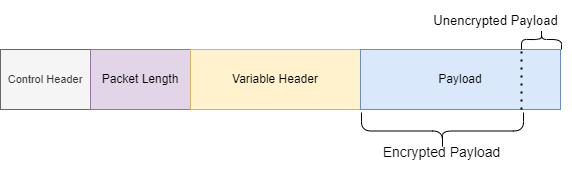
\includegraphics[width=\linewidth]{images/fp/mqttprotocol.drawio.png}
    \caption{MQTT Protocol Header Structure and Payload Encryption}
    \label{fig:mqtt}
\end{figure}

Figure \ref{fig:mqtt} shows the standard MQTT protocol header along with application message payload. Within the MQTT payload section, two distinctive parts can be identified. The first part consists of an encrypted message utilizing one of the AEAD (Authenticated Encryption with Associated Data) encryption family methods. For this particular study, both ASCON and AES-GCM encryption methods are implemented and compared. The second part of the payload contains the associated data. In this context, the device ID serves the purpose of retrieving the appropriate symmetric key by the receiver, thereby ensuring the message's authenticity and integrity.


